
\newcommand{\NbasesV}{\textit{N}}
\newcommand{\Nbases}{6}
\newcommand{\Nml}{6}
\newcommand{\NmlT}{5}
\newcommand{\NmlA}{2}
\newcommand{\Ncb}{4}
\newcommand{\MML}{método multirrótulo}
\newcommand{\MMLs}{métodos multirrótulo}
\newcommand{\MRLM}{Recursive Dependent Binary Relevance}
\newcommand{\MRLMa}{RDBR}

\chapter{Introdução}
\begin{verbatim}
 -Falar um pouco sobre aprendizado de máquina.
 -Falar sobre Classificação multiclasse
 -Apresentar Classificação multirrótulo e falar como é mais tenso que a multiclasse, dar exemplos etc.
 -Falar um pouco do estado da arte da Classificacao multirrotulo.
 
\end{verbatim}



\section{Motivações}
% A análise dos métodos multirrótulo traz os seguintes benefícios:
O melhor entendimento do funcionamento dos métodos multirrótulo permite:
\begin{itemize}
 \item descobrir atributos destes que se alterados, aproveitados
 e/ou combinados podem acarretar na criação de novos métodos e/ou na melhora dos existentes.
 \item prever, com uma certa taxa de erro, seus desempenhos, o que facilita o uso mais inteligente dos métodos
 sem precisar utilizar muito esforço computacional devido a testes.
 \item reforçar ou contrariar as conclusões já estabelecidas dos métodos, uma vez que a maioria delas são 
 baseadas em testes experimentais.
\end{itemize}

\section{Objetivos}
O objetivo geral deste trabalho é analisar e comparar métodos multirrótulos distintos e 
desenvolver um novo algoritmo de classificação multirrótulo.
Mais formalmente, a análise deve implicar em conclusões matemáticas ou estatísticas sobre o desempenho dos métodos multirrótulo.
O Objetivo geral pode ser detalhado nos seguintes objetivos específicos:
\begin{itemize}
 \item Comparação estatística e análise crítica dos métodos multirrótulos;
 \item Elaboração de um algoritmo de um novo método multirrótulo.
 \item Implementação dos métodos multirrótulos em uma biblioteca que integra técnicas de reconhecimento de padrões.
\end{itemize}


% \section{Contribuições}
\section{Estrutura do Trabalho}

\chapter{Classificação multirrótulo}

\section{Enunciado do problema}
\begin{verbatim}
ESBOÇO:
-Definição formal.
-um classificador multirrótulo mapeia do espaço de características
para um vetor de valores reais entre 0 e 1 
de tamanho igual ao número de rótulos.
-falar da complexidade do problema
-falar sobre lidar o problema como probabilidade condicional dado o rótulo e etc...
    P(l_1 | x,l_2)
\end{verbatim}



\section{Avaliação de Desempenho}
\begin{verbatim}
ESBOÇO:
-Apresentar matematicamente o que pode indicar correlação entre rótulos e outras coisas
conforme o artigo: "Bayes Optimal Multilabel Classification via Probabilistic Classifier Chains".
-Falar que é diferente do multiclasse e a razao disso
\end{verbatim}
\subsection{Métricas}
\label{sec:metrics}
\subsubsection{Accuracy}
\subsubsection{Hamming-Loss}
\subsubsection{Subset Accuracy}
\subsubsection{Example Based Accuracy}
\subsubsection{Ranking Loss}
\subsection{Modelo de Avaliação}
\label{sec:modelav}

\begin{verbatim}
ESBOÇO:
Falar do Holdout,Cross-validation estratificado.
Falar sobre bases separadas de treino,teste e validação.
\end{verbatim}

\chapter{Métodos Multirrótulos}
\section{Transformação do Problema}
\subsection{Relevância Binária - BR}
\label{sec:br}
\subsection{Classifier Chain}
\subsection{Ensemble of Classifier Chain}
\subsection{Probabilistic Classifier Chain}
\subsection{Relevância Binária Dependente - DBR}
\label{sec:dbr}
\subsection{Monte Carlo Classifier Chain}

% \section{Adaptação de classificadores}
% \subsection{ML-KNN}
% \subsection{Rede Neural Artificial}
% \subsection{C4.5 multirrótulo}
% \subsection{CRankSVM}
% \subsection{MAIS...}


\chapter{Recursive Dependent Binary Relevance - RDBR}
A proposta de \MRLM~(\MRLMa)~é fundamentada no \MML~\textit{dependent binary relevance} (DBR) \cite{dbr2014}, que é explicado
na seção \ref{sec:dbr}. Assim como o DBR e o CC, o \MRLMa~é um método baseado na transformação do problema que dividem o problema
multirrótulo em vários problemas classificação binária. Todos eles exploram a correlação entre os rótulos por meio da adição de
características especiais que representam os rótulos reais ou estimativas dos rótulos reais ao espaço de características original. 
Mas, diferentemente dos outros, o \MRLMa~adiciona uma inteligência na adição dessas características especiais na fase de predição do método.
A forma de como isso é feito, bem como o funcionamento completo do algoritmo de classificação e a fundamentação teórica
do \MRLMa~são detalhados na seção \ref{sec:mrlm_algo}. 
A seção \ref{sec:mrlm_analise} analisa o funcionamento e o desempenho do \MRLMa~de forma empírica.


\section{Algoritmo de \MRLM~-~\MRLMa}
\label{sec:mrlm_algo}
Como foi dito anteriormente, o \MRLM~é baseado no DBR. 
% Ambos se baseiam na expansão do espaço de características
% com características que representam a estimativas dos rótulos como forma de explorar
% a correlação entre rótulos. Isso é feito usando a predição do BR no espaço de características original.
% Ou seja, 
Ambos dependem da hipótese de que as estimativas dos rótulos em $Y$ por um classificador multirrótulo $c_0$
são boas características para aprimorar as estimativas dos mesmos rótulos por um novo classificador $c_1$
e que quanto melhor forem as estimativas dos rótulos por $c_0$, melhores são as de $c_1$.
% Nesse caso, podemos dizer
% que o classificador $c_0$ é usado por $c_1$ como parâmetro para .
E ainda ambos usam o BR como classificador multirrótulo base, que servirá para realizar as primeiras estimativas dos 
rótulos.

No entanto, o \MRLMa, ao invés de usar apenas o classificador base $c_0$ como função para contruir
as características adicionais que o $c_1$ usa, como o DBR,
ele também usa o próprio $c_1$ para essa finalidade, ou seja, há uma atualização das estimativas das características
pelo próprio classificador que as usam.
A idéia é que cada vez que $c_1$ as atualiza, melhores ficam suas estimativas uma vez que ele será baseado
em estimativas melhores de rótulos do que anteriormente. 
% A alimentação é a propagação das 
% estimativas dos rótulos de um classificador multirrótulo para o espaço de características expandido de um outro, ou o mesmo,
% classificador multirrótulo.
O funcionamento do algoritmo é formalmente detalhado nas seções seguintes.

Formalmente, a estrutura do \MRLMa~é organizado da seguinte forma:
\begin{itemize}
%   \item Assim como o DBR, é composto de dois classificadores multirrotulo, o primeiro, $c_0$, é um BR
%   e o segundo, $c_1$, é um BR ligeiramente modificado, que chamaremos de $BR^*$.
  \item Assim como o DBR, é composto de um BR e um classificador multirrótulo, $c_0$ e $c_1$,
  cada um composto de $l$ classificadores binários.
  \item O $c_0$ trabalha dentro do espaço de características original do problema, de nome $X$,
  e $c_1$ trabalha dentro de um novo espaço de características do problema, de nome $X_e$ e
   definido como $X_e=X \times \{0,1\}^{l}$. Assim, $c_0$ e $c_1$ são
  representados pelas seguintes funções:
  \begin{equation}
  \begin{split}
   & c_0 : X \rightarrow \{0,1\}^l \\
   & c_1 : X_e \rightarrow \{0,1\}^l
   \end{split}
  \end{equation}
  \item Os $l$ classificadores binários $c_1^1,c_1^2...,c_1^l$ que compoêm $c_1$ não trabalham no mesmo
  espaço de características, contudo,
  trabalham com uma dimensão reduzida, em $X \times \{0,1\}^{l-1}$. Digamos que $(x,y)$ seja uma instância de $X_e$
  onde $x \in X$ e $y \in {\{0,1\}}^l$, então cada instância 
  do classificador binário $c_1^i$ tem $|x|+l-1$ características e é definido como sendo $(x,y_1,...,y_{i-1},y_{i+1},...,y_{l})$.

  
%   e o resultado da classificação multirrotulo de $c_1$ é construido da seguinte forma:
%   $c_0(x,y)=(c_1^1(x,y_2$
%   \item O método contém duas funções $t_0$ e $t_1$ que mapeiam espaços de características:
%    \begin{equation}
%  \begin{split}
%     & t_0 : X \rightarrow X_e \\
%     & t_1 : X_e \rightarrow X_e \\
%     & t_0(x)=(c_0(x)) | x \in X \\
%     & t_1(x,y)=(c_1(x,y)) | x \in X,  y \in [0,1]^{l}
% %   h_i : \mathbb{R}^l \rightarrow \mathbb{R}^l & | i=1,...,n-1
%   \end{split}
%  \end{equation}
%   
  
\end{itemize}
  A figura \ref{fig:mrlm_struct} exibe uma imagem que permite visualizar a estrutura do \MRLMa.
  As seções seguintes formalizam e detalham tanto a fase de treinamento quanto a fase de predição do algoritmo.
  É importante observar que a fase de treinamento do \MRLMa~é exatamente o mesmo do que o DBR.
  A diferença de ambos os métodos se dá na fase de predição, descrita na seção \ref{sec:mrlm_prediction}.
 
 
 \subsection{Fase de Treinamento}
  A fase de treinamento do \MRLMa~é exatamente igual ao DBR.
  
  De forma mais formal, o treinamento de \MRLM~funciona da seguinte forma.
  Dado uma base de dados de treino $D=\{((x_i),y_i)|i=1,...,n\}$ onde $x_i \in X$ e $y_i \in Y$,
  primeiro treina-se o $c_0$
  no espaço de características original conforme o treinamento do próprio BR mostrado na seção \ref{sec:br}.
%   Depois, treina-se $c_1$ em uma nova base de dados $D'$ que é construída a partir de $D$ e que é
%   composta pelas instâncias $\{(y_1),(y_2),...,(y_n)\}$ as quais são os rótulos das instâncias da base de $D$
%   (ver figura \ref{fig:instsRotulos}).
  Depois, treina-se $c_1$ em uma nova base de dados $D'$ que é construída a partir de $D$ adicionando os rótulos de cada
  exemplo como características. Assim, $D'$ é composta pelos exemplos $\{((x_i,y_i),y_i) |i=1,...,n\}$ e
  cada classificador binário $c_1^j$ de $c_1$ é induzido na base de dados $D'_j=\{(x_i,y_{i,1},...,y_{i,j-1},y_{i,j+1},...,y_{i,l}),y_{i,j} | i=1,...,n\}$.
  Note que a característica representando o $j$-ésimo rótulo é removido da base de dados.
  Dessa forma, ao invés de estimar apenas $P(y_j|x)$ como o BR faz, o método é capaz de detectar dependência entre os rótulos ao
  estimar $P(y_j|x,y_1,...,y_{j-1},y_{j+1},...,y_l)$.
 
 \subsection{Fase de Predição}
 \label{sec:mrlm_prediction}
 O funcionamento do \MRLMa~distingue-se do DBR apenas na fase de predição.
 Dado uma instância $x$ onde $x\in X$ e seu conjunto de rótulos reais $y,y \in {\{0,1\}}^l$, queremos que a função $C:X\rightarrow Y$,
 representando o classificador multirrótulo \MRLMa, retorne $y$ quando o submetemos $x$, ou seja, $C(x)=y$.
 
 Como no caso do DBR e do Classifier Chain, os rótulos reais $y$, que são usado como características especiais,
 estão disponíveis apenas durante a fase de treinamento. Dessa forma, para tornar possível a classificação por $c_1$, usou-se o $c_0$ para
 estimar os rótulos, %  Para alcançar isso, o \MRLMa~, após treinado, usa $c_0$ para realizar as primeiras estimativas dos rótulos,
 resultando em $c_0(x)=\hat{y}^0=(\hat{y}_1^0,\hat{y}_2^0,...,\hat{y}_l^0)$, que servirá como parte da instância de $c_1$
 no lugar de $y$. 
 A partir daí, $c_1$ classifica a instância $(x,\hat{y}^0)$ de uma forma bem similar ao BR:
 cada classificador binário do método é responsável pela predição de um rótulo da instância.
%  \begin{equation}
%   c_1(x)=(c_1^1(x),c_1^2(x),...,c_1^l(x))
%  \end{equation}
 No entanto, o \MRLMa~adota uma técnica extra, inspirada no Classifier Chain que consiste em, para
 cada classificador binário $c_1^j$, atualizar a característica $\hat{y}_j$ imediatamente após 
 a sua classificação. Dessa forma, os classificadores binários seguintes, $c_1^{j+1},c_1^{j+2},...,c_1^{l}$,
 classificarão suas instâncias baseados em estimativas de rótulos mais atuais, possivelmente melhores.

 Assim que $c_1$ classifica a instância $(x,\hat{y}^0)$, gerando portanto a estimativa de rótulos $\hat{y}^1=c_1(x,\hat{y}^0)$,
 $\hat{y}^1$ é usado para atualizar as características da instância $x$, tomando assim o lugar de $\hat{y}^0$.
 Esse processo de atualização das características é iterativo e é repetido $r$ vezes,
 onde $r$ é determinado por um valor máximo de iterações, definido a priori, ou quando é detectado a convergência.
 A convergência é alcançada quando a estimativa de rótulos não muda, independente do número de iterações.
%  Isso acontece, por exemplo, quando $c_1(c_1(c_0))=c_1(c_0)$.
 Com $r$ iterações, tem-se $r$ estimativas de rótulos $\hat{y}^1,\hat{y}^2,...,\hat{y}^r$, dentre as quais o último ($\hat{y}^r$)
 é a classificação final do método $C(x)=\hat{y}^r$.
 
 Dessa forma, podemos concluir que \MRLM~é um método recursivo de tal forma que
 para $r=1$, $C(x)=c_1(c_0(x))$,
 para $r=2$, $C(x)=c_1(c_1(c_0(x)))$,
 para $r=3$, $C(x)=c_1(c_1(c_1(c_0(x))))$ e assim por diante.
 Note que para $r=0$, o \MRLMa~é exatamente o BR, $C(x)=c_0(x)$.
%  a aplicação de $c_1$ $3$ vezes sobre
%  $c_0(x)$ resulta na estimativa $\hat{y}^3=c_1(c_1(c_1(c_0(x))))$ e assim por diante.
 Aplicando esse processo recursivo, espera-se que a cada recursão $i$ a estimativa dos rótulos $\hat{y}^i$ seja melhor do que
 seu antecessor $\hat{y}^{i-1}$. Teoricamente, essa afirmação se mantém se supormos que a estimativa $\hat{y}^1$ é melhor do que a $\hat{y}^0$, 
 o que é razoável uma vez que o classificador $c_0$, que é um BR, obtem seu resultado usando apenas estimativas marginais dos rótulos,
 (??REFERENCIAR A EQUACAO DE PROBABILIDADE MARGINAL??)%  ($P(y|x)=\prod_{j=1}^l{P(y_j,x)}$)
 , enquanto que $c_1$ explora a correlação dos rótulos ao usá-los como características, obtendo assim 
 estimativas baseadas na probabilidade condicional.
 Com essa suposição teríamos que $\hat{y}^i$ seria melhor do que $\hat{y}^{i-1}$, pois $\hat{y}^{i-1}$ se aproxima
 mais da distribuição real dos rótulos do que $\hat{y}^{i-2}$. Assim, quando $c_1$ estimar $\hat{y}^i$ usando $\hat{y}^{i-1}$ estaria baseado em 
 uma distribuição mais próxima daquela em que foi treinado do que usando $\hat{y}^{i-2}$.
 Lembrando que $c_1$ foi treinado usando rótulos assumidamente corretos.
 
 Olhando por esse procedimento, o \MRLMa~pode ser simplesmente visto como uma generalização do BR e do DBR
 que insere uma inteligência
 adicional a aplicação e uso do classificador $c_1$ de DBR, afim de que ele seja melhor aproveitado.
 
 
 
 \section{Análise}
 \label{sec:mrlm_analise}
 \begin{verbatim}
 ESBOÇO:
  -Listar as hipoteses/suposições em que MRLM é baseado.
  -Mostrar experimentos/gráficos que comprovam que as hipoteses bases
      são verdades(geralmente).
  -Mostrar complexidade algorítma.
  -Conclusão rápida em relação a mudança que o MRLM faz com o DBR.
      (Conclusão mais detalhada será feita no último capitulo da monografia!)
 \end{verbatim}
 
 Nessa seção o método \MRLMa~é posto em prova. Com objetivo de analisar o método, implementou-se o algoritmo
 na linguagem de programação Java e no Weka \cite{weka}, que é uma biblioteca que integra técnicas de reconhecimento de padrões.
 A principal hipótese em que o \MRLMa~é baseado será testado nessa seção com o intuito de validar o método.
 Com a finalidade de tornar os testes mais objetivos, a hipótese é melhor formalizado:
 \begin{itemize}

  \item Dados uma métrica $M$, uma base de Teste $D=\{x_1,x_2,...,x_n\}$,
  um DBR induzido composto pelos classificadores multirrótulos $c_0$ e $c_1$ e
  dois vetores de predições de $l$ rótulos:
  \begin{equation}
  \begin{split}
  & p=(p_1,p_2,...,p_n) : p_i \in {\{0,1\}}^l |1 \leq i \leq n \\
  & b=(b_1,b_2,...,b_n) : b_i \in {\{0,1\}}^l |1 \leq i \leq n
  \end{split}
  \end{equation}
  tal que $M(p_2) \geq M(p_1)$,
  então:
  \begin{equation}
  M((c_1(x_i,p_1) | 1 \leq i \leq n)) \leq M((c_1(x_i,p_2) | 1 \leq i \leq n))
  \end{equation}
 
 \end{itemize}

De uma forma bem resumida e informal, a hipótese é que erros de predições pelo
classificador $c_0$ do DBR afetam negativamente a classificação do classificador $c_1$.
A comprovação dessa hipótese é feita da seguinte forma. Experimentos com o \MRLMa~são realizados
usando 7 bases de dados de domínio públicos. Cada experimento consiste em medir o valor da métrica \textit{Subset Accuracy}
quando o método é submetido a validação cruzada de 10 \textit{folds}.
O experimento é repetido com o número máximo de iterações do
\MRLMa~variando de 0 a 10 (Note que para o valor 0, o \MRLMa~se torna exatamente o BR).
Ao variar esse parâmetro, espera-se que o método obtenha desempenho melhor para os valores mais altos.
De fato, é o que ocorre na maioria dos casos, apesar de que o método estabiliza/converge rapidamente em relação ao
número máximo de iterações.
O gráfico da figura \ref{fig:Gmrlm_1} é um exemplo do que ocorre em 5 dos 7 casos testados: o método tem seu desempenho melhorado
até o valor máximo de iterações chegar a 2, depois disso o método não tem seu desempenho alterado.
Portanto 2 foi o valor máximo de iterações necessárias para o método convergir nesses casos.
Nos outros dois casos o método convergiu com apenas uma iterações ou piorou 
com duas ou mais iterações. Veja os dois gráficos dos dois casos na figura \ref{fig:Gmrlm_2}.
Vale ressaltar que em 6 dos 7 casos, o método \MRLMa~conseguiu um desempenho melhor do que o DBR e em apenas um dos casos
alcançou o mesmo desempenho do DBR.


\begin{figure}[h]
\label{fig:Gmrlm_1}
\caption{Gráfico do desempenho do \MRLMa~(eixo vertical) para vários valores máximos de iterações (eixo horizontal)
representado na linha azul.
A linha em vermelha representa um limiar para o \MRLMa~cujo valor é o desempenho do DBR}
\centering
% 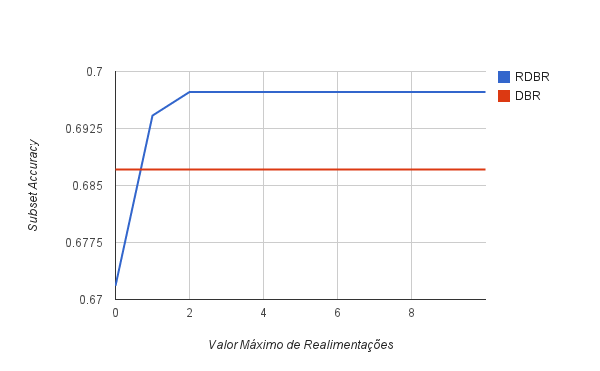
\includegraphics[width=1\textwidth] {Gmedicalj48_mrlm.png}
\end{figure}

\begin{figure}[h]
\label{fig:Gmrlm_2}
\caption{Gráficos do desempenho do \MRLMa~(eixo vertical) para vários valores máximos de iterações (eixo horizontal)
representado nas linha azuis.
A linha em vermelha representa um limiar para o \MRLMa~cujo valor é o desempenho do DBR.}
\centering
% 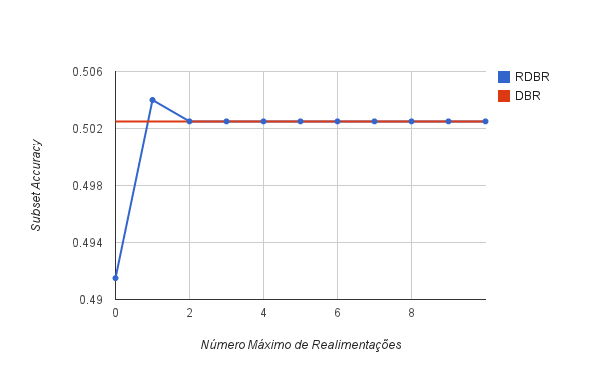
\includegraphics[width=1\textwidth] {Gbirdsj48_mrlm.png}
% 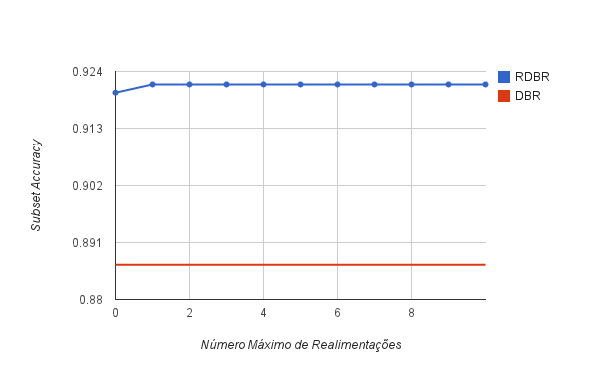
\includegraphics[width=1\textwidth] {Ggenbaseknn_mrlm.png}
\end{figure}



É importante analisar o quanto o método aumenta o tamanho da base de dados uma vez que isso acarreta no aumento
do tempo de execução do algoritmo. Seja $l$ o número de rótulos, $n$ o número de instâncias de treino
e $m$ o número de atributos da base original, na fase de treinamento do \MRLMa, o número de base de dados utilizadas são
$2l$, cada uma contendo $n$ instâncias. Em metade delas, as instâncias contidas tem $m$ atributos e na outra metade $m+l$ atributos.
Já na fase de predição do algoritmo, no pior caso, o algoritmo usa $(r+1)l$ bases de dados de $n$ instâncias onde na primeira base, o
número de atributos é igual a $m$ e nas restantes é igual $m+l$. Vale ressaltar que nem todas essas bases de dados são
armazenados explicitamente na mémoria em espaços diferentes, algumas são reutilizadas no processo de predição.

% Em relação a complexidade algorítma do \MRLMa, ela pode ser
% aproximada pelo número de atributos destinados ao classificador base, uma vez que é um método de transfomação
% e a maior parte do custo computacional se encontra no classificador base.
% A complexidade 




\chapter{Avaliação e Análise Experimental}
Nesta seção é descrito as bases de dados multirrótulo usadas nos experimentos, as medidas de avaliação escolhidas e a escolha
dos parâmetros dos classificadores. 

\section{Base de dados}
Todas as 7 bases de dados utilizadas nos experimentos foram obtidas de repositórios públicos pelo seguinte endereço virtual ??.
As bases de dados são apresentadas a seguir:

\begin{itemize}
\item \bf{Emotions}: ??
\item \bf{Scene}: ??
\item \bf{Yeast}: ??
\item \bf{Birds}: ??
\item \bf{Genbase}: ??
\item \bf{Medical}: ??
\item \bf{Enron}: ??	

\end{itemize}
\label{tab:datas}
\begin{table}[h]
\caption{Resumo das bases de dados multirrótulos}
\begin{tabular}{|c|ccccccc|}
\hline
% \textbf{}         & \textbf{}        & \textbf{}         & \multicolumn{2}{c}{\textbf{ATRIBUTOS}} & \textbf{}        & \textbf{}              & \textbf{}          \\
\textbf{BASE}     & \textbf{DOMÍNIO} & \textbf{EXEMPLOS} & \textbf{DIS} & \textbf{NUM} & \textbf{RÓTULOS} & \textbf{CARD} & \textbf{DENS} \\ \hline
\textbf{Emotions} & Música           & 593               & 0                 & 72                 & 6                & 1.869                  & 0.311              \\
\textbf{Scene}    & Imagem           & 2407              & 0                 & 294                & 6                & 1.074                  & 0.179              \\
\textbf{Yeast}    & Biologia         & 2417              & 0                 & 103                & 14               & 4.237                  & 0.303              \\
\textbf{Birds}    & Audio            & 645               & 2                 & 258                & 19               & 1.014                  & 0.053              \\
\textbf{Genbase}  & Biologia         & 662               & 1186              & 0                  & 27               & 1.252                  & 0.046              \\
\textbf{Medical}  & Texto            & 978               & 1449              & 0                  & 45               & 1.245                  & 0.028              \\
\textbf{Enron}    & Texto            & 1702              & 1001              & 0                  & 53               & 3.378                  & 0.064             \\ \hline
\end{tabular}
\end{table}

A tabela \ref{tab:datas} apresenta algumas estatísticas das bases de dados adquiridas.
Nessa tabela são apresentadas as seguintes informações de cada base de dados:
\begin{itemize}
  \item \textit{DIS}: número de atributos discretos;
  \item \textit{NUM}: número de atributos numéricos;
  \item \textit{CARD}: cardinalidade de rótulos na base de dados;
  \item \textit{DENS}: densidade de rótulos na base de dados.
\end{itemize}


\section{Método de Comparação}
\label{sec:methodcomp}
A comparação e estudo dos métodos é feita considerando o custo computacional e a qualidade de predição.
A qualidade de predição é estimada pelo método de avaliação por validação cruzada \ref{sec:modelav} com 10 grupos
(\textit{10-fold cross-validation}) sobre \Nbases~bases de dados, todas apresentadas e descritas na subseção seguinte.


Para quantificar a qualidade de predição, foram escolhidas as seguintes métricas:
\begin{itemize}
 \item Subset Accuracy, pois é mostrado que captura bem a correlação entre rótulos;
 \item Example Based Accuracy, pois é bem mais sensível que o Subset Accuracy;
 \item ??
%  \item Tempo computacional, pois é @@@ etc...
\end{itemize}

As fórmulas para o cálculo de cada uma das métricas são apresentadas na seção \ref{sec:metrics}.
É interessante mostrar os resultados experimentais usando diferentes métricas, pois cada uma captura
um aspecto diferente da classificação. 
Num total, foram utilizados \Nml~modelos de classificação multirrótulos: BR, DBR, RDBR, CC, ECC e MCC.
Para cada um deles utilizou-se os seguintes classificadores base: KNN, SVM, J48 e Regressão Logística. 
Para o melhor entendimento, neste capítulo um método multirrótulo é definido como sendo a combinação
de um modelo de classificação multirrótulo com uma configuração de parâmetros pré-definida. Assim, por exemplo,
o classificador BR com KNN é considerado um método diferente do classificador BR com SVM. Isso, por um lado é bom
pois testa o desempenho dos classificadores multirrótulo quando não é gasto tempo computacional para ajustar parâmetros.
Por outro lado é ruim uma vez que considera os mesmos modelos de classificação como sendo completamente diferentes.
Dessa forma, foram considerados 24 métodos multirrótulos e comparados entre si de forma experimental.

% 
% Este capítulo se encontra dividido em duas seções, na primeira foram analisados os
% resultados dos métodos de transfomação para cada classificador base.
% Já na segunda seção cada combinação de método multirrótulo com classificador base foi considerado
% um método de transformação e seus resultados são comparados entre si juntamente com os métodos multirrótulos
% de adaptação.


\section{Resultados Experimentais}
Nesta seção é feita uma análise geral do desempenho dos métodos multirrótulos em cada uma das bases de dados.
Para cada base de dados é apresentado uma tabela
contendo os valores das métricas escolhidas para cada um dos métodos multirrótulo e o
o ranking dos métodos multirrótulos para cada métrica.

\subsection{Emotions}

\begin{table}[h]
\label{tab:emotionsExps}

\caption{EXEMPLO DE TABELA, NAO É DE VERDADE AINDA!}

\begin{tabular}{l|llll}
                           & Hamming Loss  & Subset Accuracy & Example-Based Accuracy & \\ \hline
ECC (Logistic)             & 0.2100\textpm 0.0285 (1) & 0.2577\textpm 0.0718 (2)  & 0.5205\textpm 0.0508          &  \\
MCC (Logistic)             & 0.2323\textpm 0.0228 (3) & 0.2476\textpm 0.0466 (1)  & 0.5101\textpm 0.0425          &  \\
LabelPowerset (Logistic)   & 0.2664\textpm 0.0203 (2) & 0.2175\textpm 0.0304 (4)  & 0.4593\textpm 0.0289          &  \\
PCC (Logistic)             & 0.2277\textpm 0.0238 (6.5) & 0.2459\textpm 0.0580 (6)  & 0.5150\textpm 0.0462          &  \\
CC (Logistic)              & 0.2342\textpm 0.0274 (4) & 0.2442\textpm 0.0642 (5)  & 0.5032\textpm 0.0462          &  \\
BR (Logistic)              & 0.2193\textpm 0.0275 (12) & 0.2241\textpm 0.0555   & 0.4944\textpm 0.0410          &  \\
MRLM (Logistic)            & 0.2471\textpm 0.0183 (13) & 0.2358\textpm 0.0493   & 0.4879\textpm 0.0369          &  \\
DBR (Logistic)             & 0.2547\textpm 0.0203 (9) & 0.2038\textpm 0.0401   & 0.4851\textpm 0.0323          &  \\
ECC (J48)                  & 0.2268\textpm 0.0231 (6.5) & 0.2832\textpm 0.0417   & 0.5097\textpm 0.0442          &  \\
MCC (J48)                  & 0.2479\textpm 0.0300 (3) & 0.2427\textpm 0.0547   & 0.4826\textpm 0.0447          &  \\
LabelPowerset (J48)        & 0.2777\textpm 0.0258 (3) & 0.2056\textpm 0.0477   & 0.4369\textpm 0.0412          &  \\
PCC (J48)                  & 0.2474\textpm 0.0249 (3) & 0.2476\textpm 0.0552   & 0.4770\textpm 0.0408          &  \\
CC (J48)                   & 0.2550\textpm 0.0181 (3) & 0.2478\textpm 0.0259   & 0.4703\textpm 0.0350          &  \\
BR (J48)                   & 0.2474\textpm 0.0248 (3) & 0.1838\textpm 0.0500   & 0.4623\textpm 0.0352          &  \\
MRLM (J48)                 & 0.2612\textpm 0.0274 (3) & 0.2561\textpm 0.0506   & 0.4700\textpm 0.0431          &  \\
DBR (J48)                  & 0.2561\textpm 0.0298 (3) & 0.1737\textpm 0.0564   & 0.4402\textpm 0.0548          &  \\
ECC (IBk)                  & 0.1996\textpm 0.0235 (3) & 0.3133\textpm 0.0562   & 0.5489\textpm 0.0440          &  \\
MCC (IBk)                  & 0.2080\textpm 0.0254 (3) & 0.3403\textpm 0.0618   & 0.5676\textpm 0.0502          &  \\
LabelPowerset (IBk)        & 0.2092\textpm 0.0255 (3) & 0.3319\textpm 0.0556   & 0.5660\textpm 0.0528          &  \\
PCC (IBk)                  & 0.2016\textpm 0.0281 (3) & 0.3538\textpm 0.0656   & 0.5809\textpm 0.0523          &  \\
CC (IBk)                   & 0.2013\textpm 0.0261 (3) & 0.3421\textpm 0.0459   & 0.5765\textpm 0.0418          &  \\
BR (IBk)                   & 0.1903\textpm 0.0228 (3) & 0.3151\textpm 0.0448   & 0.5503\textpm 0.0400          &  \\
MRLM (IBk)                 & 0.2055\textpm 0.0251 (3) & 0.3420\textpm 0.0494   & 0.5749\textpm 0.0442          &  \\
DBR (IBk)                  & 0.2170\textpm 0.0201 (3) & 0.3066\textpm 0.0509   & 0.5740\textpm 0.0424          &  \\
ECC (SMO)                  & 0.1850\textpm 0.0274 (3) & 0.3337\textpm 0.0612   & 0.5794\textpm 0.0517          &  \\
MCC (SMO)                  & 0.2013\textpm 0.0262 (3) & 0.3284\textpm 0.0618   & 0.5747\textpm 0.0482          &  \\
LabelPowerset (SMO)        & 0.2252\textpm 0.0263 (3) & 0.2696\textpm 0.0457   & 0.5320\textpm 0.0432          &  \\
PCC (SMO)                  & 0.2038\textpm 0.0221 (3) & 0.3335\textpm 0.0569   & 0.5755\textpm 0.0407          &  \\
CC (SMO)                   & 0.2038\textpm 0.0251 (3) & 0.3100\textpm 0.0570   & 0.5558\textpm 0.0446          &  \\
BR (SMO)                   & 0.1909\textpm 0.0244 (3) & 0.2933\textpm 0.0381   & 0.5408\textpm 0.0449          &  \\
MRLM (SMO)                 & 0.2047\textpm 0.0207 (3) & 0.3437\textpm 0.0643   & 0.5783\textpm 0.0419          &  \\
DBR (SMO)                  & 0.2156\textpm 0.0273 (3) & 0.3101\textpm 0.0494   & 0.5849\textpm 0.0403          & 
\end{tabular}
\end{table}

\subsection{Medical}
\subsection{Yeast}
\subsection{Scene}
\subsection{Genbase}
\subsection{Enron}
\subsection{Birds}

\section{Complexidade Algorítima}




\chapter{Conclusão}